
\section{Experiments}
\label{sec:exp}

In this section, we evaluate our method on real datasets. We
implemented our method in Java language. We ran our experiments on Java
runtime environment version 1.6 on Linux machines with 2.2-GHz dual AMD Opteron
dual core processors, and 3 GBs of main memory.

\paragraph{Datasets}
In our experiments, we used two datasets of protein interactions
in Homo Sapiens and Rattus Norvegicus from MINT\cite{mint1} (the Molecular
INTeraction database). The first one is a large dataset of 15472 interactions
among 6122 proteins. The second one is a smaller dataset of 806 interactions
among 631 proteins. Each interaction is described by two interacting proteins and a
reliability score between 0 and 1 that represents the level of confidence that
this interaction truly exists. MINT calculates reliability scores of
interactions using a heuristic formula of available evidence, including the
size and type of the experiment reporting the interaction, sequence similarity
of ortholog proteins and the number of publications supporting the
interaction\cite{mint2}. 

We use the negative logarithm of MINT reliability scores as edge weights. In all
experiments, we find pathways starting within the set of membrane proteins and
ending within the set of transcription factors. We use the Gene Ontology
database\cite{go} to identify membrane proteins and transcription factors of each
dataset. We identify membrane proteins as the ones under the terms GO:0005886
and GO:0004872, and transcription factors as the proteins under the terms
GO:0000988, GO:0001071 and GO:0006351.

\subsection{Performance assessment and comparison}


\begin{figure}[h]
\centering
\subfigure[H.sapiens, path length = 6]{
	\label{iterations_hsa_6}
	\includegraphics{results/iterations/hsa6}
}
\goodgap
\subfigure[H.sapiens, path length = 8]{
	\label{iterations_hsa_8}
	\includegraphics{results/iterations/hsa8}
}
\subfigure[R.norvegicus, path length = 6]{
	\label{iterations_rat_6}
	\includegraphics{results/iterations/rat6}
}
\goodgap
\subfigure[R.norvegicus, path length = 8]{
	\label{iterations_rat_8}
	\includegraphics{results/iterations/rat8}
}
\caption{Confidence level acheived after a given number of iterations,
comparing our method to Scott et al. and empirical confidence. X-axis is the
number of iterations finished, and Y-axis is the level of confidence in the
optimality of the result, for H.sapiens and R.norvegicus at different path
lengths. The empirical line denotes the observed probability that the optimal
path is found at or before a given iteration, averaged over several experiments.}
\label{iterations}
\end{figure}



We run an experiment to measure how fast the value of confidence rises with each
iteration in both our method and the one presented by Scott et al.\cite{scott}.
We run each method for 500 iterations and measure the overall confidence after
each iteration is finished. We also compare these results with the empirical
confidence, which is the probability of finding the optimal pathway as
empirically observed. To compute the empirical confidence, we run 500
coloring iterations and assign each iteration a value $s \in \{0, 1\}$, where
$s = 1$ if the optimal pathway is found in this iteration or in a preceding one,
and $s = 0$ otherwise. We repeat this experiment multiple times and take the
average values of $s$ for each iteration as the empirical confidence of this
iteration. Figure \ref{iterations} shows the confidence value as more iterations
finish, for our method and Scott et al. and also the empirical confidence value.
The figure shows a gap between Scott et al. confidence and empirical confidence,
which is expected because of the conservative way they use to calculate success
probability of an iteration, as discussed in section \ref{background}. This gap
increases as the path length parameter increases. Our method closes this gap and
produces confidence values that are closer to the empirical confidence values.
The figure also shows that our method produces higher confidence values than
Scott et al. for the same number of iterations.

\begin{figure}[h]
\centering
\subfigure[H.sapiens, path length = 6]{
	\label{times_hsa_6}
	\includegraphics{results/times/time_hsa6}
}
\goodgap
\subfigure[H.sapiens, path length = 8]{
	\label{times_hsa_8}
	\includegraphics{results/times/time_hsa8}
}
\subfigure[R.norvegicus, path length = 6]{
	\label{times_rat_6}
	\includegraphics{results/times/time_rat6}
}
\goodgap
\subfigure[R.norvegicus, path length = 8]{
	\label{times_rat_8}
	\includegraphics{results/times/time_rat8}
}
\subfigure[R.norvegicus, path length = 9]{
	\label{times_rat_9}
	\includegraphics{results/times/time_rat9}
}
\caption{Total time needed to acheive a given level of confidence by our method
and Scott et al. X-axis is the level of confidence in the optimality of the
result, and Y-axis is the total time taken to acheive this confidence level,
for H.sapiens and R.norvegicus at different path lengths. Lower values are
better.}
\label{times}
\end{figure}



We also measure the total time taken by our method to reach a given
confidence level as opposed to that of Scott {\it et
  al.}~\cite{scott}. We run both methods for 500 iterations and
measure, after each iteration, the confidence level reached and the
overall time taken by both methods. Figure \ref{times} shows that our
method takes less time than Scott et al. to achieve the same level of
confidence. The figure also shows that the our performance lead
increases as the path length parameter increases.



\subsection{Validation Experiments}
\label{sec:validation}


So far we have shown that our method outperforms existing coloring
strategies in terms of the running time performance. In this section,
we evaluate the biological significance of the results we can find
using our method. 

It is worth mentioning that our method returns the same results as
Scott {\it et al.}~\cite{scott} when both of them are allowed to reach
a high confidence value (such as 99\% confidence). The main difference
is that our method scales to larger networks and longer paths.
Therefore, here we will only focus on the results obtained by our
method.


\subsubsection{Statistical significance of the results}
\label{sec:zscore}

%\begin{wraptable}{r}{0.40\textwidth}
\begin{table}[t]
  \tbl{$Z$-scores calculated for the optimal paths found by our method for
  H.sapiens and R.norvegicus for different path lengths. $Z = \frac{\mu
  - \theta}{\sigma}$ where $\mu$ is the average weight of 1000 randomly
  generated paths, $\sigma$ is their standard deviation, and $\theta$ is the
  weight of the optimal path found by our method.} {
\begin{tabular}{|l|c|c|c|c|c|c|c|c|c|}
\hline
	&	\multicolumn{9}{c|}{Path Length}		\\ \cline{2-10}
Dataset	&	\multicolumn{3}{c|}{6}	&	\multicolumn{3}{c|}{7}	&
	\multicolumn{3}{c|}{8}	\\
	\cline{2-10} 
		&	\begin{math}\mu\end{math}	&	\begin{math}\theta\end{math}	&
	\begin{math}Z\end{math} & \begin{math}\mu\end{math}	&	\begin{math}\theta\end{math}	&
	\begin{math}Z\end{math} & \begin{math}\mu\end{math}	&
	\begin{math}\theta\end{math}	& \begin{math}Z\end{math}	\\ \hline
{\it H.sapiens}	&	5.906	&	0.129	&	5.409	&	7.074	&	0.130	&	5.477	&	8.341	&
0.221	&	5.764	\\
{\it R.norvegicus}	&	4.975	&	4.540	&	0.889	&	7.307	&	5.025	&	1.453	&
8.457	&	4.858	&	1.467
\\
\hline
\end{tabular}
}
\label{tab:zscore}
\end{table}
%\end{wraptable}

In this section we assess the statistical significance of the paths found of our
method; how our results compare to random paths. We use $Z$-score to
measure statistical significance. For each dataset and path length, we run our method to
get the path with the minimum weight $\theta$. we then generate 1000 random
simple paths that start at a membrane protein and end at a transcription
factor. We compute the average weight $\mu$ of these random paths and their
standard deviation $\sigma$. We then compute the $Z$-score as follows
\begin{equation}
Z = \frac{\mu - \theta}{\sigma}
\end{equation}
$Z$-score indicates by how many standard deviations our optimal weight is
better than the weight of an average random path, so higher values are better.
Table~\ref{tab:zscore} shows $Z$-scores for H.sapiens and R.norvegicus for path
length 6, 7 and 8. Our results are always better than the random ones.
The calculated $Z$-scores range from 0.89 to 5.76. It can also be observed that,
for a given dataset, $Z$-score increases with increasing the path length, which
is expected because increasing the size of random selection leads to less
chances of the selected path being better or closer to the optimal path.
From these observations observations, we can infer that our results are
statistically significant.


\subsubsection{Biological significance of the results}

\begin{wrapfigure}{r}{0.50\textwidth}
  \centering
  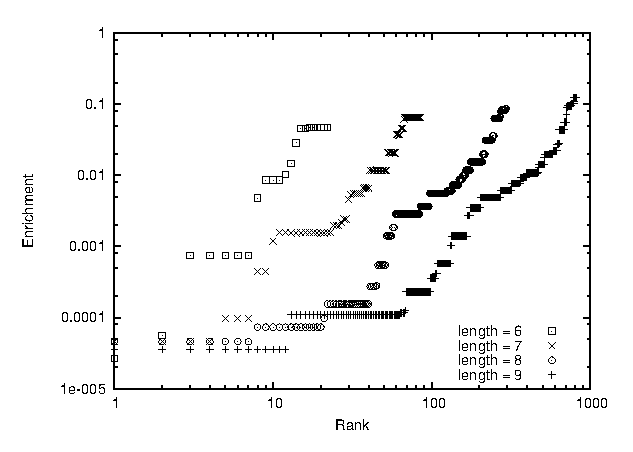
\includegraphics[width=0.45\textwidth]{results/enrichment/enrich-rank}
  \caption{Sorted values of functional enrichment of optimal and suboptimal
  paths found at different iterations of our method. X-axis is the rank of the
  path with regard to its functional enrichment in log scale, and Y-axis is the
  enrichment value of this path. Lower values are better.}
  \label{fig:enrichment-rank}
\end{wrapfigure}


\begin{wrapfigure}{r}{0.50\textwidth}
  \centering
  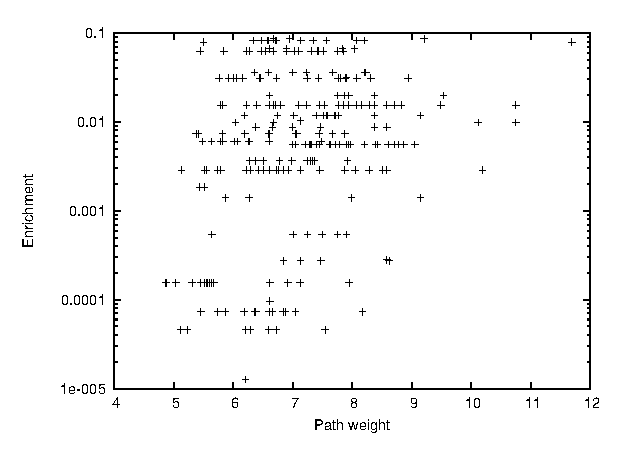
\includegraphics[width=0.45\textwidth]{results/enrichment/enrich-score}
  \caption{Functional enrichment values of paths against their weights. X-axis
  is path's weight and Y-axis is its corresponding enrichment value. Lower
  values are better.}
  \label{fig:enrichment-score}
\end{wrapfigure}


Another important question is: how biologically significant are our results? To
answer this question, we validate our results using functional enrichment. We
use the Gene Ontology\cite{go} to compute functional enrichment of paths found
at different iterations of our method. Let $\Phi$ be the path being tested, $T$
be the universal set of GO terms, $m$ be the path length, $M$ be the total
number of proteins in the dataset, $G_i$ be the total number of proteins
annotated with the Go term $t_i$ in the dataset, and $g_i$ be the number of
proteins annotated with $t_i$ in $\Phi$. We compute functional enrichment of
$\Phi$ as $\min_{t_i \in T} P(X \geq g_i | M, m, G_i)$ where $X$ is a random
variable under under a hypergeometric distribution with these parameters. Lower
values of are better.



 
\subsection{Discussing paths found}
 
 \begin{figure}[h]
\centering
\subfigure[All proteins annotated by GO:0042058 - regulation of epidermal growth
factor receptor signaling pathway]{
	\label{fig:path_go0042058}
	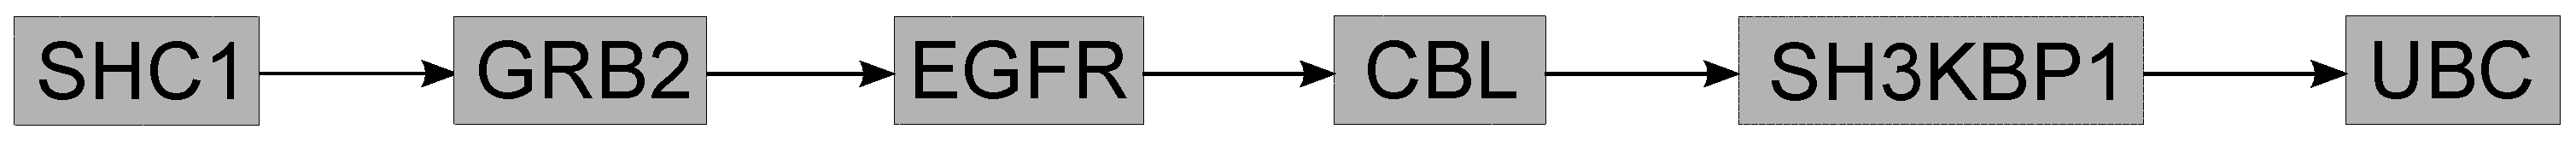
\includegraphics[width = 0.8\textwidth]{figures/path_go0042058}
}
\subfigure[First five proteins annotated by GO:0042059 - negative regulation of
epidermal growth factor receptor signaling pathway]{
	\label{fig:path_go0042059}
	\includegraphics[width = 0.8\textwidth]{figures/path_go0042059_2}
}
\subfigure[All proteins annotated by GO:0046875 - ephrin receptor binding]{
	\label{fig:path_go0046875}
	
\includegraphics[width = 0.8\textwidth]{figures/path_go0046875}
}
\caption{Caption goes here}
\label{fig:paths}
\end{figure}
 
